\documentclass[12pt,oneside,a4paper]{article}
\usepackage[utf8]{inputenc}
\usepackage{booktabs}
\usepackage{float}
\usepackage{graphicx}
\graphicspath{ {./images/} }


\title{Acceleration and Braking Recognition}
\author{Felipe Bombardelli}
\bibliographystyle{plain}


\begin{document}

\maketitle

\section{Introduction}

The work aims to recognize the sound of train, when they braking or accelerating, from a WAV file using SVM and Convolution Neural Network (CNN) like classifier. There is no work about train recognizing on the IEEEXplorer, but there some works about environmental sound recognition \cite{chachada-survey}\cite{huzaifah-features}.



\section{Program Structure}

The code of solution was divided on 3 modules for a better organization and reuse of code. The first module called datasetmod is responsible by handle and normalize the dataset. The second, way\_classic is responsible by training and evaluation classic classifiers like KNN, Neural Network and SVM. And by last, way\_cnn is responsible by training and evaluation  classifier using CNN.


\section{Dataset and Data Normalize}

The dataset has 2996 samples with one channel and rate 22050 Hz divided by 9 classes, as shown in the table \ref{tab:dataset}.
How the samples of dataset have different duration, so it needs to divide the samples in little window with same size.

\begin{table}[H]
	\centering
	\begin{tabular}{@{}llll@{}}
		\toprule
		Id & Label                      & Samples  & Average Duration \\ \midrule
		0  & negative/checked           & 828      & 9.83             \\
		1  & accelerating/1\_New        & 493      & 3.57             \\
		2  & accelerating/2\_CKD\_Long  & 169      & 3.57             \\
		3  & accelerating/3\_CKD\_Short & 74       & 3.56             \\
		4  & accelerating/4\_Old        & 410      & 3.38             \\
		5  & braking/1\_New             & 381      & 4.58             \\
		6  & braking/2\_CKD\_Long       & 143      & 4.51             \\
		7  & braking/3\_CKD\_Short      & 62       & 4.35             \\
		8  & braking/4\_Old             & 436      & 3.95             \\ \bottomrule
	\end{tabular}
	\label{tab:dataset}
	\caption{Dataset provided}
\end{table}

According the work \cite{huzaifah-features} there are some representation used to learning features like short-time Fourier transform (STFT) with linear and Mel scales, constant-Q transform (CQT) and continuous Wavelet transform (CWT). And Mel-STFT, STFT and CQT were consistently good performers \cite{huzaifah-features}. In this work, the descriptor used was the Mel-Scaled Spectrogram through the function librosa.feature.melspectrogram() provided by the Librosa library.




\subsection{Methodology}

The work evaluates 2 CNN architecture, SVM, KNN and Neural Network. For evaluating, the dataset was divided in 70\% to train and 30\% to test. The first CNN architecture is called in this work by CNN-flat and it similar a Neural Network. The second CNN architecture is called CNN-based-piczak and based on the work \cite{huzaifah-features}, which is described in the figure \ref{fig:model}. Finally the CNN models were trained using 10 epochs.

\begin{figure}
	\centering
	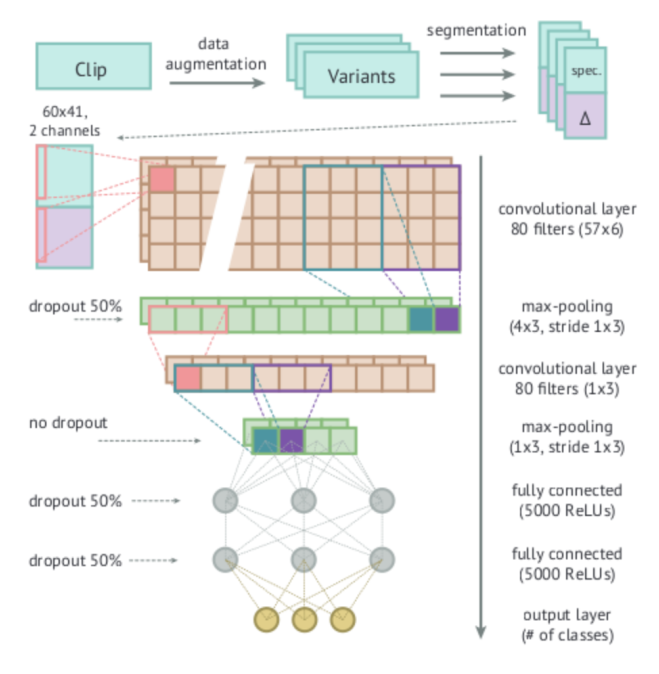
\includegraphics[scale=1.0]{model.png}
	\caption{CNN Architecture used in the work \cite{piczak} }
	\label{fig:model}
\end{figure}


It performs some tests to choice the window size and frequency resolution needed to mel-scale. The tests consist in train a CNN-flat varying the resolution frequency and window size, and analyzing their accuracy tested on the 30\% of the dataset.
Firstly, the window size was fixed in 175(4s), because the 5 classes in the dataset has less than 4s of duration and the frequency resolution was varied from 10 until 40. So the table \ref{tab:frequency} shows, that frequency resolution greater 20 don't improve more the accuracy.

\begin{table}[H]
	\centering
	\begin{tabular}{@{}lll@{}}
		\toprule
		Frequency Resolution  &   Window Size    & Accuracy \\ \midrule
		10                    & 175 (4s)          & 0.8254  \\
		15                    & 175 (4s)          & 0.8756  \\
		20                    & 175 (4s)          & 0.8876  \\
		25                    & 175 (4s)          & 0.8869  \\
		30                    & 175 (4s)          & 0.8939  \\
		35                    & 175 (4s)          & 0.8869  \\
		40                    & 175 (4s)          & 0.8939  \\  \bottomrule
	\end{tabular}
	\label{tab:frequency}
	\caption{Result of the test varying the frequency resolution}
\end{table}

After defined the frequency resolution in 25, also it was realized same tests to define a good window size. So the window size was variable from 50(1.1s) until 200(4.6s). When the sound have duration next to the window size, so the sound is padding or cutting, else the sound is divided in many windows. In the table shows \ref{tab:window}, that the frequency resolution greater than 150 don't improve more the accuracy. Therefore, the window size adopted was 150.

\begin{table}[H]
	\centering
	\begin{tabular}{@{}lll@{}}
		\toprule
		Frequency Resolution  &   Window Size    & Accuracy   \\ \midrule
		25                    & 50   (1.1s)      & 0.83     \\
		25                    & 75   (1.7s)      & 0.83     \\
		25                    & 100  (2.3s)      & 0.87     \\
		25                    & 125  (2.9s)      & 0.88     \\
		25                    & 150  (3.5s)      & 0.89     \\
		25                    & 175  (4.0s)      & 0.88     \\
		25                    & 200  (4.6s)      & 0.89     \\  \bottomrule
	\end{tabular}
	\label{tab:window}
	\caption{Result of the test varying the window size}
\end{table}



\section{Results and Discussion}

The evaluating of the classifiers used 25 frequency resolution and window size of 150 as parameter. So the table show the accuracy obtained for each classifier. The result CNN-flat and Neural Network had the best accuracy.

\begin{table}[H]
	\centering
	\begin{tabular}{@{}ll@{}}
		\toprule
		Label              & Accuracy   \\ \midrule
		CNN-flat           & 0.8933     \\
		CNN-based-piczak   & 0.8251     \\
		SVM                & 0.8718     \\
		KNN                & 0.8379     \\
		Neural Network     & 0.8939     \\ \bottomrule
	\end{tabular}
	\caption{Accuracies of the classifiers using frequency resolution=25 and window size=150}
\end{table}

Although the result of CNN-flat was 0.89, when the classifier was aplied in the real-world scenario, it don't have apparently the same accuracy, how showed in the figure \ref{fig:result_real}. Because in the same braking or accelerating have multiples classes of the trains.

\begin{figure}[H]
	\centering
	
\includegraphics[scale=0.6]{result1.png}
	\caption{ Result using CNN-flat classifier on the file test\_files/tram-2018-11-30-15-30-17.wav. Green means a train accelerating and Red means a train braking. The different tons of the greens and red are different classes of the trains. }
	\label{fig:result_real}
\end{figure}


\section{Conclusion}
	The accuracies on the tests on 30% of the dataset was good, but this same result don't appear in the real scenario. Maybe using 2 classifier, the first only classifies between accelerating or braking, and the second classifier the type of the train. So it is possible to avoid to classify different trains classes for the same braking or accelerating. Other detail, that can to improve the result, is balance the amount of samples of the classes to train the classifier.


\bibliography{research}

\end{document}
